%%%%%%%%%%%%%%%%%%%%%%%%%%%%%%%%%%%%%%%%%
% Wenneker Assignment
% LaTeX Template
% Version 2.0 (12/1/2019)
%
% This template originates from:
% http://www.LaTeXTemplates.com
%
% Authors:
% Vel (vel@LaTeXTemplates.com)
% Frits Wenneker
%
% License:
% CC BY-NC-SA 3.0 (http://creativecommons.org/licenses/by-nc-sa/3.0/)
% 
%%%%%%%%%%%%%%%%%%%%%%%%%%%%%%%%%%%%%%%%%

%----------------------------------------------------------------------------------------
%	PACKAGES AND OTHER DOCUMENT CONFIGURATIONS
%----------------------------------------------------------------------------------------


\documentclass[11pt]{scrartcl} % Font size
%%%%%%%%%%%%%%%%%%%%%%%%%%%%%%%%%%%%%%%%%
% Wenneker Assignment
% Structure Specification File
% Version 2.0 (12/1/2019)
%
% This template originates from:
% http://www.LaTeXTemplates.com
%
% Authors:
% Vel (vel@LaTeXTemplates.com)
% Frits Wenneker
%
% License:
% CC BY-NC-SA 3.0 (http://creativecommons.org/licenses/by-nc-sa/3.0/)
% 
%%%%%%%%%%%%%%%%%%%%%%%%%%%%%%%%%%%%%%%%%

%----------------------------------------------------------------------------------------
%	PACKAGES AND OTHER DOCUMENT CONFIGURATIONS
%----------------------------------------------------------------------------------------

\usepackage{amsmath, amsfonts, amsthm} % Math packages

\usepackage{listings} % Code listings, with syntax highlighting

\usepackage[english]{babel} % English language hyphenation

\usepackage{graphicx} % Required for inserting images
\graphicspath{{Figures/}{./}} % Specifies where to look for included images (trailing slash required)

\usepackage{booktabs} % Required for better horizontal rules in tables

\numberwithin{equation}{section} % Number equations within sections (i.e. 1.1, 1.2, 2.1, 2.2 instead of 1, 2, 3, 4)
\numberwithin{figure}{section} % Number figures within sections (i.e. 1.1, 1.2, 2.1, 2.2 instead of 1, 2, 3, 4)
\numberwithin{table}{section} % Number tables within sections (i.e. 1.1, 1.2, 2.1, 2.2 instead of 1, 2, 3, 4)

\setlength\parindent{0pt} % Removes all indentation from paragraphs

\usepackage{enumitem} % Required for list customisation
\setlist{noitemsep} % No spacing between list items

%----------------------------------------------------------------------------------------
%	DOCUMENT MARGINS
%----------------------------------------------------------------------------------------

\usepackage{geometry} % Required for adjusting page dimensions and margins

\geometry{
	paper=a4paper, % Paper size, change to letterpaper for US letter size
	top=2.5cm, % Top margin
	bottom=3cm, % Bottom margin
	left=3cm, % Left margin
	right=3cm, % Right margin
	headheight=0.75cm, % Header height
	footskip=1.5cm, % Space from the bottom margin to the baseline of the footer
	headsep=0.75cm, % Space from the top margin to the baseline of the header
	%showframe, % Uncomment to show how the type block is set on the page
}

%----------------------------------------------------------------------------------------
%	FONTS
%----------------------------------------------------------------------------------------

\usepackage[utf8]{inputenc} % Required for inputting international characters
\usepackage[T1]{fontenc} % Use 8-bit encoding

\usepackage{fourier} % Use the Adobe Utopia font for the document

%----------------------------------------------------------------------------------------
%	SECTION TITLES
%----------------------------------------------------------------------------------------

\usepackage{sectsty} % Allows customising section commands

\sectionfont{\vspace{6pt}\centering\normalfont\scshape} % \section{} styling
\subsectionfont{\normalfont\bfseries} % \subsection{} styling
\subsubsectionfont{\normalfont\itshape} % \subsubsection{} styling
\paragraphfont{\normalfont\scshape} % \paragraph{} styling

%----------------------------------------------------------------------------------------
%	HEADERS AND FOOTERS
%----------------------------------------------------------------------------------------

\usepackage{scrlayer-scrpage} % Required for customising headers and footers

\ohead*{} % Right header
\ihead*{} % Left header
\chead*{} % Centre header

\ofoot*{} % Right footer
\ifoot*{} % Left footer
\cfoot*{\pagemark} % Centre footer
 % Include the file specifying the document structure and custom commands


%----------------------------------------------------------------------------------------
%	TITLE SECTION
%----------------------------------------------------------------------------------------

\title{	
	\normalfont\normalsize
	\textsc{Universidad Central del Ecuador}

	\textsc{Facultad de Ingeniería y Ciencias Aplicadas}

	\textsc{Carrera de Ingeniería Informática}
	\vspace{6pt} % Whitespace
	\rule{\linewidth}{0.5pt}\\ % Thin top horizontal rule
	\vspace{20pt} % Whitespace
	{\huge Desarrollo de una Aplicación Móvil}\\ % The assignment title
	\vspace{12pt} % Whitespace
	\rule{\linewidth}{2pt}\\ % Thick bottom horizontal rule
	\vspace{12pt} % Whitespace
}

\author{\LARGE Nelson Ricardo Baquero} % Your name

\date{\normalsize\today} % Today's date (\today) or a custom date

\begin{document}

\maketitle % Print the title

\section{Conceptualización}

\subsection{¿Qué idea de aplicación móvil tengo pensado hacer?}

Un "tracker" de tareas que ayude a construir hábitos. La idea es que el usuario pueda agregar tareas que desee realizar diariamente y la aplicación lleve un registro de los días en los que se completaron, además de generar un calendario que presente la información de forma intuitiva y amigable.


%------------------------------------------------
%----------------------------------------------------------------------------------------
%	TEXT EXAMPLE
%----------------------------------------------------------------------------------------

\subsection{¿En qué tipo de aplicaciones me he basado?}

Existen varias aplicaciones en las tiendas que permiten seguir tus hábitos, pero la mayoría carece de ayudas visuales que pienso proporcionar, además de ser de pago. Otra gran inspiración es el calendario de contribuciones de GitHub que muestra de forma visual cada día donde se realizó commits y la cantidad.

\begin{figure}[h] % [h] forces the figure to be output where it is defined in the code (it suppresses floating)
	\centering
	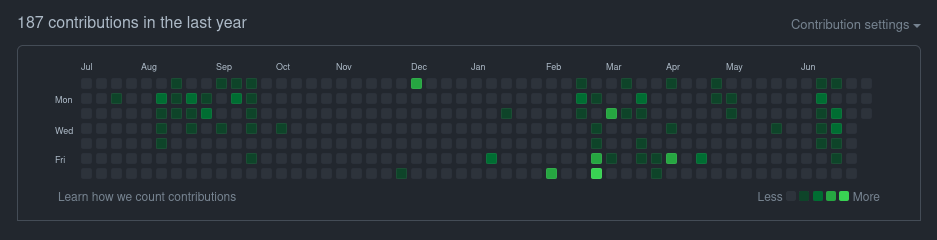
\includegraphics[width=\columnwidth]{github_contributions.png} % Example image
	\caption{Calendario de contribuciones de GitHub.}
\end{figure}

\subsection{¿Cuáles son los aspectos actuales de la tecnología e innovación que han inspirado esta aplicacion?}

Con la cantidad de distracciones que existen en internet, hoy en día es muy difícil formar nuevos hábitos. La idea es utilizar las capacidades de un smartphone para ayudar en la formación de dichos hábitos, por ejemplo con el uso de notificaciones push, base de datos interna y sincronización con un servidor externo.

\subsection{¿Qué necesidades voy a cubrir cuando mi aplicación esté funcional?}

El usuario podrá:
\begin{itemize}
	\item Registrar hábitos, colocar horarios y repeticiones diarias o semanales.
	\item Generar un plan diario de tareas a cumplir.
	\item Recibir notificaciones push con recordatorios de sus tareas diarias.
	\item Visualizar su progreso de manera visual con gráficos.
\end{itemize}

\subsection{¿En qué categoría está ubicada mi aplicación?}

Salud y productividad.

\section{Definición}

\subsection{¿Qué tipos de usuarios usarán mi aplicación?}

Según las estadísticas de Google Play, existen alrededor de 100.000 aplicaciones en la categoría de productividad, volviéndola parte del top 10 de categorías según el número de aplicaciones. La conclusión es que existe un mercado importante de usuarios que sienten importante el uso de aplicaciones para mejorar su productividad. En el campo de salud, existen cerca de 90.000 aplicaciones.

\begin{figure}[h] % [h] forces the figure to be output where it is defined in the code (it suppresses floating)
	\centering
	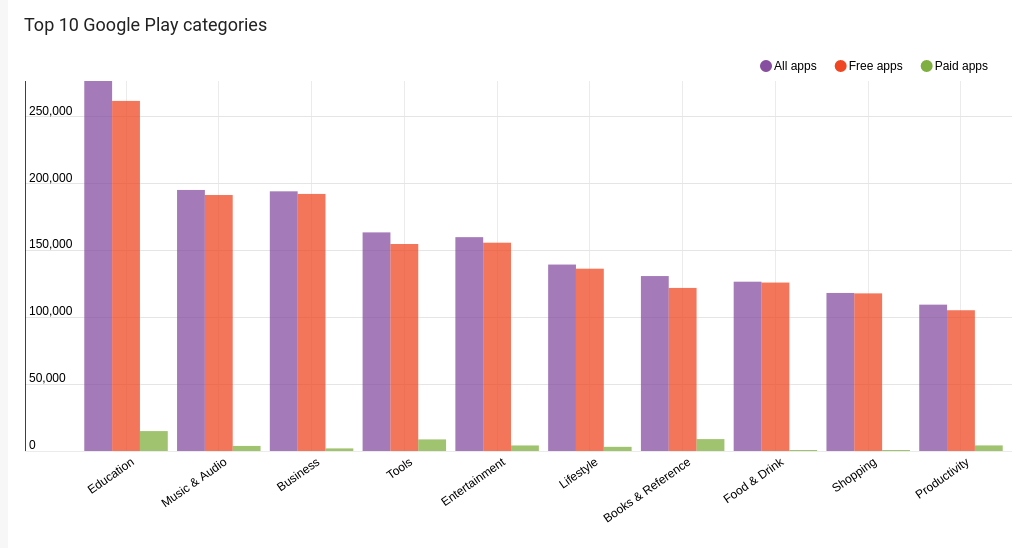
\includegraphics[width=\columnwidth]{google_play_stats.png} % Example image
	\caption{Top 10 categorías según el número de aplicaciones. Excluye juegos.}
\end{figure}

\subsubsection{¿Qué segmento poblacional será el primero en usarla?}

Usuarios jóvenes-adultos entre 18 y 30 años que busquen desarrollar nuevos hábitos con un horario apretado o con una cantidad inmensurable de distracciones a las que estamos sometidos diariamente con internet.

\subsection{¿Qué acciones podrán realizar mis usuarios cuando usen mi aplicación?}

\begin{enumerate}
	\item Al abrir la aplicación serán recibidos con una vista de calendario mostrando las tareas cumplidas en el mes y las tareas a realizar en el día.
	\item La siguiente pantalla permitirá agregar nuevas tareas y configurar su tipo de repetición, horario, notificaciones, cantidad de tiempo a dedicar, entre otros.
	\item Permitirá visualizar estadísticas de cumplimiento semanal o mensual de cada tarea.
\end{enumerate}

\subsection{¿Qué funcionalidades no estarán presentes en mi aplicación cuando esté lista para su uso?}

\begin{itemize}
	\item Gráficos estadísticos (como barras o dispersión) de las tareas cumplidas.
	\item Recomendaciones sobre tareas adicionales o tips para completarlas.
\end{itemize}

\subsection{¿Qué partes o secciones tendrá mi aplicación?}

\begin{figure}[h] % [h] forces the figure to be output where it is defined in the code (it suppresses floating)
	\centering
	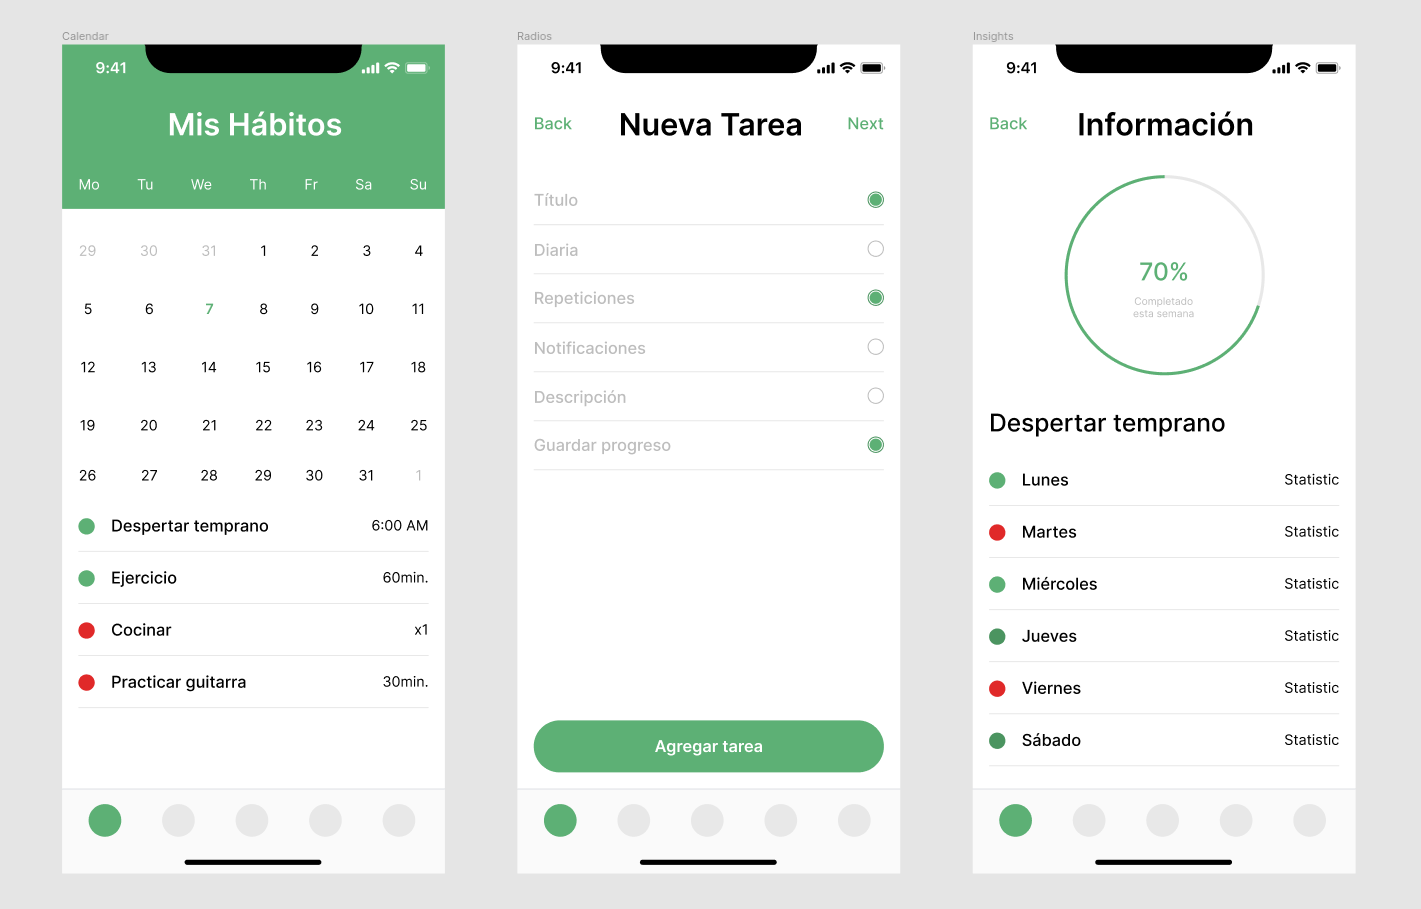
\includegraphics[width=\columnwidth]{app_diseno.png} % Example image
	\caption{Ejemplo de funcionalidades de la aplicación.}
\end{figure}

\pagebreak

\section{Diseño}

\subsection{¿En qué aplicación me basaré para generar mi diseño?}

Principalmente en el calendario de contribuciones de GitHub.

Para la lista y seguimiento de tareas, la aplicación recordatorios de iOS es un buen punto de inspiración.

\begin{figure}[h]
	\centering
	\begin{subfigure}{.5\textwidth}
		\centering
		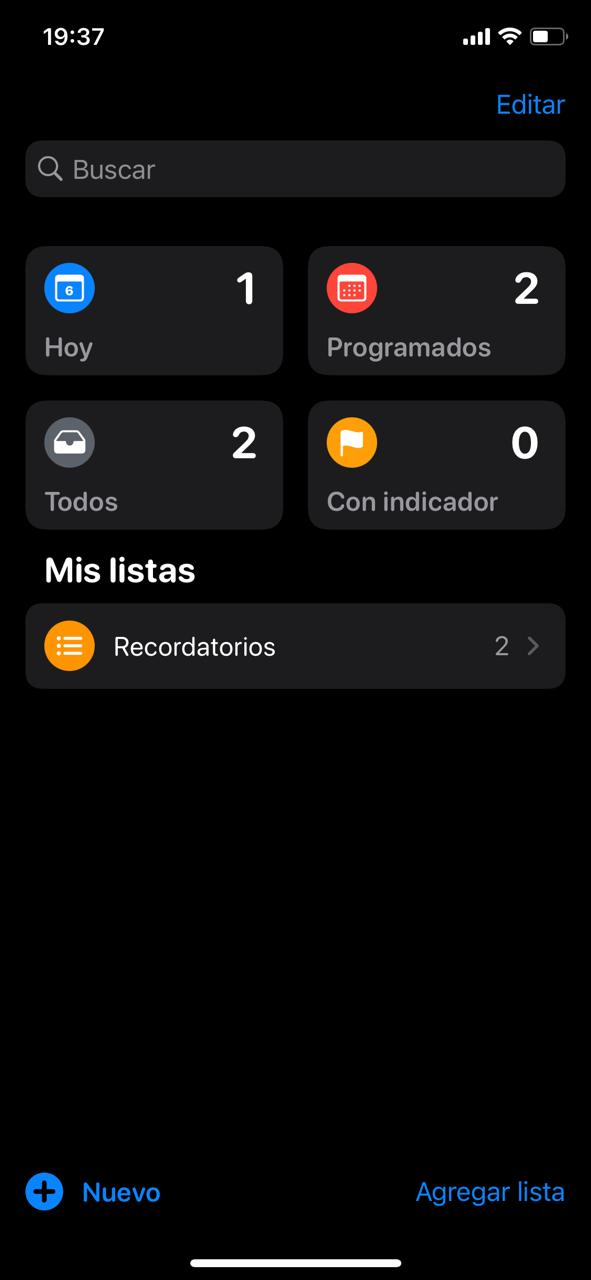
\includegraphics[width=.6\linewidth]{recordatorios_1.jpeg}
		\caption{Vista inicial de app Recordatorios.}
		\label{fig:sub1}
	\end{subfigure}%
	\begin{subfigure}{.5\textwidth}
		\centering
		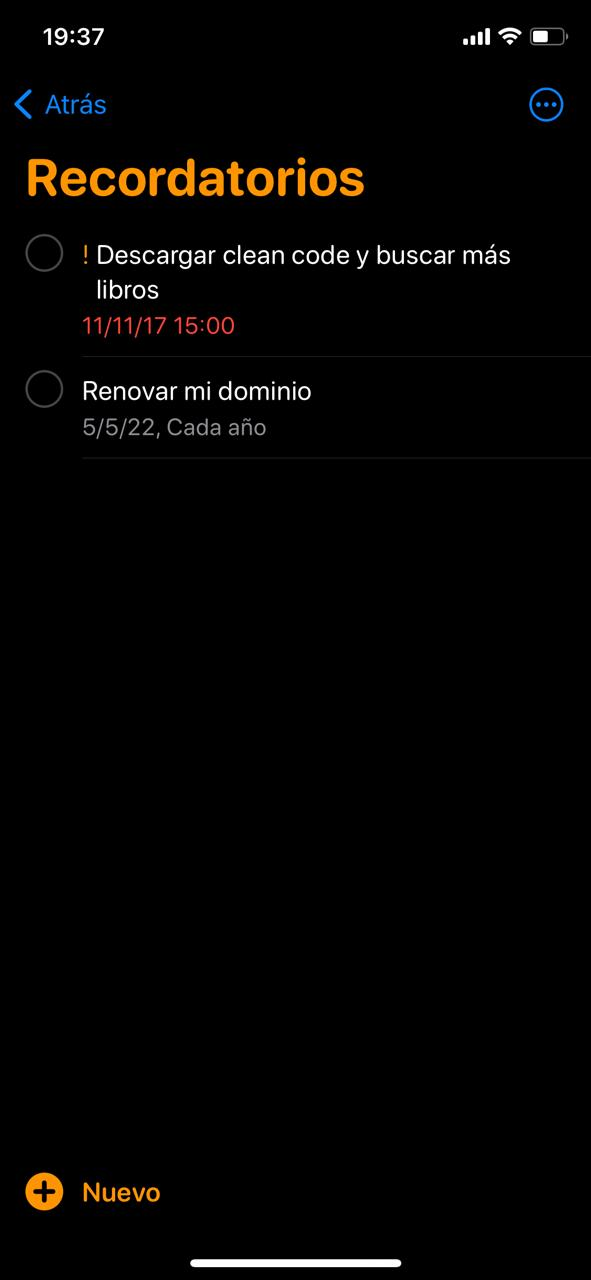
\includegraphics[width=.6\linewidth]{recordatorios_2.jpeg}
		\caption{Lista de recordatorios.}
		\label{fig:sub2}
	\end{subfigure}
	\caption{Aplicación Recordatorios de iOS.}
	\label{fig:test}
\end{figure}

\end{document}
